\documentclass[12pt]{article}
\usepackage[english]{babel}
\usepackage[utf8x]{inputenc}
\usepackage{apacite}
\usepackage[a4paper,width=155mm,top=25mm,bottom=25mm]{geometry}
%\usepackage{setspace}
%\doublespacing
\usepackage{graphicx}
%\graphicspath{ {graphics/} }

% Keywords command
\providecommand{\keywords}[1]{\textbf{\textit{Keywords---}} #1}
% Quotation command
\providecommand{\quotes}[1]{``#1''}
\providecommand{\singlequotes}[1]{`#1'}

\title{Thesis Draft}
\author{Mustafa İlhan}

\begin{document}
\maketitle

%%%
%%%
%%%
\begin{abstract}
In this thesis (re-)usage of discarded materials in the process of art making and the artwork itself is explored (or researched). Why and how are they used by the artist? Are there any differences with the original items compared to discarded items? (In other words using has using discarded materials or trash specific (or special) meaning and message?) This is a work to explore the re-usage of trash in artworks (place or the role in the art practice). (and also in which scope? medium, message, life practice\ldots) 

Actually (It is questioned that) working with trash dictates a life practice and, it is a convergence of behavioral patterns (attitudes toward to trash) and art making. The process effects how one's lives and lifestyle. (But what type of interaction between life and art making process?) (This claim is the main driving force of my artwork which is part of a thesis.)

With the help of art discarded thing can be find a place in the society. This issue is examined through the trash which is discarded by the society. By the help of artistic approach things can be gain new values and meaning even if they are discarded and excluded from daily life. The relationship between value creation and artistic practice examined through the artworks that uses trash as medium and representation.

From periods where manual labor and long struggle required in production process and materials are reused and transformed again and again, have reached to periods where production process speeds up and becomes more accessible. Consumption habits have changed radically and have created piles of trash that is not obvious how to reuse them. In this work the practice and process of reusing and transforming trash which is an alternative to today's existing production and consumption habits is investigated. Stages and expression of this practice is examined with my artwork in the context of art.

Driving questions: Do she/he want to take back (or revisit) the trash once thrown away? People do not want to think of what they throw away. Turning them to a things that worth to look again. 
\end{abstract}
\keywords{trash, art, value creation}

%%%
%%%
%%%
\section{What is trash?}
In this thesis work to understand the different aspects of trash is a key element. Because as scholars agreed on it is part of our life and daily practice and it is very common concepts from developed western societies to rural areas, from disaster areas to \ldots(something beautiful here). Sometimes it is accepted as a problem that is need to carefully and seriously manged. On the other hand it is accepted as a source of diversity. (To establish a solid understanding for trash, it is important to see its dilemmas (it is really a dilemma?)). Therefore we should ask these questions: What is trash? How does it became trash? Is it a end product or a source material? How much is it valuable? How much is it dangerous?

%%
%%
\subsection{Trash is everywhere and, produced every time}
Modern (developed) societies are continuously generating trash and, pile them on landfills. It's a common object category that all people share its possession. During daily activities trash is generated and people get rid of them by throwing away. (Various objects become trash after their primary functions daily. Who defined the primary function? Primary function is the only function. People cares the package of the objects that they buy. They buy the coffee not the cup of it. After coffee finished the life of cup also finishes. There is a lifetime defined (or forecast) by the producer of objects. However it is not bound to the producer, also consumer play an important role. There are different choices. Throw it away. Keep it. Give it. Mostly wining choice is throwing away and by the result of it mountains of garbage are increasing.) The vast amount of industrial discarded items spread through the landfills to oceans. They are the result of highly complex industrial production methods. They are not easily disposable items. They live in the nature thousands of years. Most of them packages that are used to carry or protect other materials. After real material used these packages became valueless (or useless). (types of trash can be mentioned here, but currently in the artwork I'm using paper packages, therefore, it is more important.) How manage the all this increasing trash that damaging nature?  This is the common approach to trash and the main problem. (actually the sustainability problem.) It is not the only problem, It can be thought that it is a losing the ability to transform new things, alternative behaviors etc. (Instead of creating new opportunities or alternatives, it is a consuming all them and producing huge pile of trash.) (reference Zizek idealization of nature, to love nature is to love trash. Live with trash. Do not see it as trash actually. Then the question is how to love trash? how to live with trash? can living with our trash enrich (our perceptions, abilities)? how not to see them as trash and useless? Can it be possible with art?)

% TODO PRAP. REF.
Waste pickers are an important part of the story in Latin America, as more is being thrown away than ever. The World Bank estimates that the amount of solid waste generated in cities is growing faster than the rate of urbanization. The higher the income level and the rate of urbanization, the greater the amount of solid waste produced. OECD countries produce almost half of the world’s waste. Africa and South Asia produce the least waste. High-income countries have the highest collection rates and are most likely to dispose of waste to landfills or incinerators. Low-income countries have the lowest collection rates and are most likely to dispose of their waste in open dumps. However, low-income countries also have the largest numbers of informal waste pickers who collect, sort, and reclaim recyclables---thus reducing costs to the city and to the environment. (FROM Trash as Treasure, BY WILLIAM L. FASH AND E. WYLLYS ANDREWS)

% TODO PRAP. REF.
Literature is recycled material, a pretext for making more art. I learned this distillation of lots of literary criticism in workshops with children. I also learned that creative and critical thinking are practically the same faculty, since both take a distance from found material and turn it into stuff for interpretation. For a teacher of literature over a long lifetime, these are embarrassingly basic lessons to be learning so late, but I report them here for anyone who wants to save time and stress. (FROM Recycle the Classics, BY DORIS SOMMER)

% From Beautiful Trash Art and Transformation BY PAOLA IBARRA ReVista
% TODO PRAP. REF.
We relate to garbage daily. We use it, produce it and dispose of it. Endlessly. The most obsessive of us get rid of it as fast as we can. The hoarder likes to salvage a few things for later use---the plastic and glass containers, the cardboard boxes. We know that capitalism’s escalating cycles of production, consumption and obsolescence keep worsening an already problematic relationship between humankind, waste and nature (not to mention social and economic relations). Despite a relatively increased awareness about consumption and its consequences, the pace at which we also acquire and dispose of material objects is exploding. Particularly in the connection between
garbage and the arts, I am interested in two questions. First, the issue of recycling as a general practice in the arts; and secondly, in the whole issue of representation---that is, representation of waste as subject, and representation (of waste or others subjects) through waste as material. (BY PAOLA IBARRA)

%
\subsubsection{Cycle of trash}
Trash moves, objects moves from place to place. From homes to garbage trucks. From streets to land fills. From garbage baskets to sculptures. [REF. MIT Garbage project] Lots of different people touches to trash. With the trash what moves?

% <From "Trash Moves On Landfills, Urban Litter and Art" by Maite Zubiaurre
Below part Explains journey of trash, its different steps. Object moves and also trash also moves. How is it life of trash? This part explains life of trash. How does it intersect with other people in which places? This part also can be understand by pointing out different part of it with detailed explanation. For example an artist collect from trash from streets and the other one goes to the (For example Vik Muniz) landfill. In other words there are different places to touch on trash. Every place generates different story? Or to understand it more deeply it covers different part of it. Or provides ideas about it. Lots of people touches it from philosophers to artist. Also in the later parts it draws attention to them. [PRAP, REF Maite Zubiaurre]

Trash moves, all the time. It becomes a steadily growing heap of clutter behind closed walls, accumulates and festers under tight lids, travels from a small trash can in the kitchen to a large one on the curbside, joins other people’s rubbish when the garbage truck arrives, drives to the transfer station, where it circles around on conveyer belts, bids farewell to recyclable or compostable goods, is loaded (if declared useless: the ultimate trash) into yet another garbage truck, or barge, or even train, until it arrives at its final destination: a sanitary landfill. Even in the landfill, it does not remain still. Monster "waste handling dozers" move rubbish around, compact it and press it against the soil. More importantly, they incessantly “sculpt” refuse with their huge shovels and caterpillar wheels, making sure the garbage mound does not tip over to create a fetid avalanche. When night falls, and the trash load of the day finally disappears under a thick layer of mud, detritus still moves: once underground, it settles differently, and decomposes at a different speed, thus continuously altering landfill topography: where there was an even plateau, now there is an abruptly descending slope, and a valley; and where there was a perfectly smooth road, now there are deep crevices in the pavement. This is how trash moves. But\ldots who moves on trash? In the United States, it is mostly big-wheeled machines, an industrious army of giant yellow insects busying themselves on a heap of rubbish. In Latin America, it is mostly people. People who hand-pick garbage, who build their shacks on densely compacted trash layers, and who, day in and day out, eagerly throw themselves into the boisterous cascades of fresh debris falling from garbage trucks. In many of the garbage dumps around the world, scavenging becomes a steady job. \quotes{Garbage properly \quotes{stored} and put away brings peace of mind, as do corpses boxed and buried, or criminals confined to a cell.} And
thanks to Art: for Art shows how trash--even the one that stops moving, and particularly the one that lies squished, squashed, and weathered, almost fossilized, on the ground---has the potential to move: to move us, that is. (through the works of Filomena Cruz's photographic series “Road Kill”) [PRAP, REF Maite Zubiaurre]
% >

%
\subsubsection{Examined-life, Zizek}
(There is a curious fragment where Zizek, dressed as a sanitation man, stands in a waste deposit in a pile of garbage and ponders over garbage and human existence. In documentary film, Examined-life, Zizek talks about ecology in the middle of a garbage dump in London, and his part starts with these sentence: "This---garbage dump--- is where we should start feeling at home". He asserts his claim at first and go through explaining how ecology turns to ideology and mentions wrong perception about the ecology. Draw attention to notion of even if trash disappears from our world but not world. It seems as though the thrown out garbage disappears from
our world. However, it disappears only from the world of illusions, but still exists in reality. He thinks that the way of approaching ecology is problematic, because accepting that nature as a balanced harmonious thing. He claims that it is ideological in the sense that wrong thinking important problems. Nature contains unimaginable catastrophes. think oil and distinct animals and plants. we profit balance part of the nature but it is created from catastrophe. Are we aware of this catastrophe. He asserts that ecology will slowly turn to religion that "is a kind of an unquestionable highest authority." Ideology of ecology warns us like, "Don't do that. It would be too much." its voice is like "Don't mess with D.N.A. Don't mess with nature. Don't do it" etc. We should not forget that we are part of the ecology. We must more alienated from the nature. We must find poetry and spirituality in the dimension of trash. That's the true love of world. Love is not about idealization. This part will be extended later.)

\quotes{According to Zizek, modern understanding of ecology is the real false consciousness, connected with mystification of real problems. Postmodern mysticism arises when disasters begin to be rationalized, interpreted in strict logic terms of cause-effect relations. Such interpretation makes life easier. However, nature is not an absolute balance and total harmony (this aspect of Zizek’s thought makes him akin to classical conservatives). Nature is a series of unthinkable disasters. Zizek believes that ecology is transforming into a new western conservative ideology: “One should not play games with nature! Do not touch DNA! Do not develop new medicines! Do not invent new technologies!” How one should react to these reproaches? Zizek’s recipe is to reinforce alienation from nature, to become more artificial.} \cite{vafin2012zizek}

His basic argument is that the modern eco movement is a conservative ideology. It says don't do X from an authoritarian high ground and it idolizes and mystifies ecology. Basically he says the eco movement has it's head in the clouds. If it loved the environment it would recognize the rubbish we create and the chaotic nature of ecological change and try to further divorce itself from that process(nature) and try to turn the whole thing into art. 

\begin{itemize}
\item Our relation to our filth follows an “out of sight, out of mind” principle, but trash doesn’t disappear.
\item Ideology addresses real problems but mystifies them.
\item We search for meaning when a horrible event happens to make it easier to accept.
\item The ideology of ecology is that world is in the best possible state and that humans disturb nature.
\item Nature is not an organism in balance that humans exploit, but rather a series of great catastrophes.
\item Ecology is becoming more like religion with dogmas.
\item Even if we learn the potential catastrophes of nature, we ignore them as long as they don’t manifest near us.
\item The solution is not to worry about saving nature, but to figure out how to survive without it by becoming more artificial.
\item Learn to love our trash as a part of ecology.
\end{itemize}	

How much harmonious all these produced materials with nature? How many animals and the plant can use these discarded items? (Because of complex production methods their recycling requires complex processes again. Some of them already produced to protect goods from natural factors (like decaying etc.). However how can we protect nature from them?) It is very hard that spontaneously they become harmonious with nature. However, some artists turned to trash into site-specific sculptures that are more than trash heap. not discarding but bracing our attitudes turned them to a something that worth it to watch and think about it. (Converting what we create harmonious with the existing system.) Because it is not possible to think that nature will live harmoniously what we created. The more likely idea will be we will live harmoniously with what we create.

Getting rid of it is not the significant action. It still waits us at somewhere else or the next generations have to cope with it. (Establish relationship with the afterthought.) Maybe the first thing to do is accept the trash, to accept that there are things out there that serve nothing. To break out of this eternal cycle of functioning.

The issue of trash is not limited with ecological and economic perspective, it has also other dimensions.(draw attention to multidimensionality of this topic, but why? and what are the other dimensions?)

Trash itself is not the only problem, the practice, lifestyle causing it is more important problem. The dynamics of market and flow of objects into it plays important role production of trash.

Trash of developed societies has higher decomposing period in the nature. Therefore results in higher damage to the nature, hard to reuse, hard to transform, sometimes not to safe to keep them because toxic elements etc. 

%
\subsubsection{Perspectives related with trash from different disciplines}
\begin{itemize}
\item Ecological perspective: Trash causes ecological problems and it treats the balance of nature. Animals do not aware of plastics materials and they unconsciously eat them.
\item Management of it handled by generally by the municipals. 
\end{itemize}

\quotes{We live in a badly engineered world, because the vast amounts of waste (both material and energetic) are needless; and that waste could be virtually eliminated through better design} \cite{mcdonough2010cradle}. In other word the problem is our technology which is not perfect. (and I'm not sure that at some point that technology will reach to the perfection or not.)

\quotes{As I prepared this issue of ReVista, some have asked me if Bogotá’s garbage crisis inspired the theme. Yes and no.  After Christmas, I traveled with a group of friends to the Chocó, an isolated and impoverished region on Colombia’s Pacific Coast. Christmas decorations abounded, and I noticed they were almost all crafted from used tin cans, old newspapers, discarded textiles and found wood objects. No one called it recycling. Trash was to be used and used again.}\cite{} Already a group of people live with their trash, what is problematic is here global ruling consumerist is not live with their trash. They can not handle their trash. There is no place for trash in their life.

\quotes{There’s a relationship between graveyards and landfills, one that makes us uncomfortable, Zubiaurre explained. \quotes{What is happening to trash is what is going to happen to us. We’re all going to end up in a dump, and we’re going to decompose. That’s the ultimate destiny of humankind, and we don’t want to face that.} Trash is also regarded differently, depending on where you live. Last year, an undergrad in Zubiaurre’s honors collegium seminar went to a poor neighborhood and scavenged through people’s trash; no one cared, Zubiaurre said. But when the same student went to Beverly Hills to go through trash, the police were nearly called. \quotes{Who decides what is public and what is private? How come trash becomes highly private in a rich neighborhood, but truly disposable in a poor neighborhood?} Zubiaurre said.} \cite{}

WALL-E is a 2008 American computer-animated science-fiction comedy film produced by Pixar Animation Studios. A robot named WALL-E, who is designed to clean up an abandoned, waste-covered Earth far in the future. WALL-E resembles to giant dozers that moves and piles trash in the landfills. 

%
\subsubsection{Throw away culture}
Continuously consuming things and disposing of something. It is an important concept to understand why trash is trash? (or how it become trash?) Behavioral pattern of throw away culture results in the trash. (This pattern does not consider recycling of it.) Artworks that are trying to raise awareness is related with this concept.

(Our trash generating behavioral daily consumption patterns \ldots What are the results of them? Why are they throwing?) (There is a behavior that throws away and opposite of it there is a collecting behavior.) 

%
\subsubsection{How does it become trash?}
Here the purpose is to understand the dynamics that turn objects to trash. By understanding them is provide a roadmap (or ideas) how to turn trash to something valuable? (The purpose of this thesis is to find (or explore) a way(methodology, approach) to add value to object using artistic methods? Therefore first question is why they are less-valued, and ignored. How to make them valuable? How to make them part of our life again?)

%
\subsubsection{Comparison of trashes}
The complexity of produced trashes of societies is increasing. For example developed countries that have nuclear plant generates radioactive wastes which highly hazardous for the environment is never exist previous societies. Think batteries and so on. Every society generates different types of wastes. Differs from country to country, society to society, ages to ages.

It can be thought that when the complexity of trashed increased required effort to repair, reuse and recycle is also increase. Therefore for the ones that have no complex tools it is becoming harder to reuse objects. In other words objects become more complex their re-usage becomes less likely. 

%
\subsubsection{Types of trashes}
Different production process generates different types of trash. According to production process, decomposition process\ldots

%
\subsubsection{What is wrong with trash?}
Relationship between entropy (second law of thermodynamics) and waste. Resources of nature turns to waste that it can revert it. Creating that are reversible again is problematic through the nature of sustainability. What is produced after it is consumed become worthless. 

From my point of view and approach in this thesis, trash is only one of the thing that is being discarded by humans and communities. There are lots of things that are being excluded such as homosexuals, trans, disabled peoples etc. Even if they are excluded, there is also life for them. 

% TODO Reference
John Scanlan's book, On Garbage shows how western progress always has cleared away and discarded what went before; not only material waste but also knowledge. He believes that by examining our garbage we can gain useful insight into the condition of contemporary life.

% TODO motivations of artists. their ideas about them, because they also point what is wrong with it? or their perceptions that 

%%
%%
\subsection{Collecting trash}
One of the most important parts of the using trash in the artwork (or expressing something, or representation) is to collect them. What are the dynamics(considerations) of collecting them? (easily accessible materials or unique items.) Where to store them? Does it mean that live with trash? In other words collecting trash and using them is live with them? (making them part of life.) After the being part of the are they still trash? Can be thought that it is something that affects the lifestyle. (possessions and trash.) Another question is that how differs collecting trash from collecting other things such as objects that have archival value. What is the driving force? You may collect it to prevent object being lost. For archival things what you collect is something that has some sort of social use and meaning which is going to disappear. However, trash is never disappearing, even its amount increasing rapidly. For archival things people have memories with them, but does some applies for the trash? Who wants to keep trash? or who wants to re-see(re-visit) trash again (in a museum for example)?

%
\subsubsection{The case of \quotes{The Gleaners and I}}
The Gleaners and I is a 2000 French documentary film by Agnès Varda that features various kinds of gleaning. The Gleaners and I is notable for its fragmented and free-form nature along with it being the first time Varda used digital cameras. This style of film making is often interpreted as a statement that great things like art can still be created through scraps, yet modern economies encourage people to only use the finest product.

It's a self-reflexive film because the director establish a relationship with the practice of gleaners and her film making practice. Some people gleans crops, the others discarded food, the other baby dolls and Agnès Varda gleans images.  

\quotes{Agnès Varda’s film, The Gleaners and I, documents the history and current practice of gleaning in France. Historically, gleaning is the act of collecting leftover crops from farmers’ fields after the harvest. However, in the film Varda expands this definition to include actions that are presently coined \quotes{dumpster diving} where people collect any types of rubbish or unwanted items to reuse them in their own way. Moreover, Varda includes her actions of collecting images with a video camera as gleaning. She is gleaning images. The Gleaners and I far more than document the lives of gleaners. It highlights the degree of global consumerism of the modern world and the ways art can exist within it in relation to gleaning.}

The official subject of this film is gleaning, the act of gathering remnants of crops from a field after the harvest. As Varda demonstrates, people can be discovered throughout the French countryside gleaning everything from potatoes to grapes, apples to oysters, much as they did hundreds of years ago (though no longer in organized groups). More figuratively, there are also urban gleaners who salvage scraps from bins, appliances from the side of the road, or vegetables from stalls after the markets have closed. And then there’s Varda herself, a gleaner of images, driving around France with a digital camera and a tiny crew (at times, she wields a smaller camera herself, permitting an even greater degree of intimacy).

Making use out of something that has been left behind and labeled as obsolete is not unique to farms and crops. There is so much discarded, yet still-viable food in dumpsters that many people live off it entirely. Seeing the value in what someone else has defined as trash is an art in itself.

Once as a common practice of gleaning throughout the years has evolved, but not disappeared. She keeps light to the modern life gleaners that are not visible every time. One of the interesting thing is here Agnès Varda feels that as a aging person will later become discarded person. In other word we can be subject of the refusal. At some point she become the subject of the thing that she track. 

There are many aspects of this documentary film. First draw attention the practice of gleaning. The discarded items that are not fit in the industrial standards because of their shape, color etc. Even if these items are discarded and we are not aware of them, there is also another life for them. Modern life gleaners feed from them. In another words someones trash becomes another trash. There are people live the boundaries of consumption societies. They create their life from the unwanted items. what the society refuses, they find a life or create a life from them. Their lifestyle is also can be seen as alternative to the life on the urban areas with deep relationship with the consumerism. (as also Zizek mentions that love is not idealization. But the industrial processes has some standards and beyond that standards there is not a place for everyone. Life is being lived in the cites is somehow idealized life or tried to be idealized life. beyond the border of the urban there is new life generated. What is not succeed in the cities succeed outside of it.)

She uses unconsciously recorded pieces in the film. \quotes{The last definition of gleaning, gleaning images, ties into what I found both the most amusing and perplexing scene in the film. It is the scene where Varda had forgotten to turn her camera off and accidentally films the ground and her lens cap bouncing along as she walks. She sets this scene to a jazz soundtrack. While watching the scene I was certainly confused. Why is this in here? What does this have to do with gleaning? And certainly why did the scene last so long? But there was also something lovely about it. Maybe it was the music, but for some reasons my senses found it audibly and aesthetically pleasing. I wasn’t able to make much sense out of the meaning behind this scene; I believe Varda referred to it as \quotes{the dance of the lens cap}.  Luckily, Ruth Cruickshank’s article, The Work of Art in the Age of Global Consumption: Agnes Varda’s Les Glaneurs et la glaneuse (The Gleaners and I), addressed this scene and clarified the potential deeper meaning behind it. Cruickshank likened the scene to something that is normally thrown away, or in this case edited out of the film, much like the way trash is thrown away or food is left behind after a harvest. Varda gleans the image of the dancing lens cap, \quotes{Where many documentary makers would leave such accidental footage on the cutting room floor, Varda draws attention to how what would habitually be perceived as waste may be viewed as supplement with its own intrinsic value. Rather than literally treating it like dirt, Varda retains and prompts reassessment of that which is normally left out of shot} \cite{cruickshank2007work}. Things that are often forgotten or discarded can easily be revamped to create something useful to someone. The scene was revamped using music and it became beautiful, much like the gleaners who found fish in the trash cooked it to make it edible, or the artist gleaner who piled discarded baby dolls into totem poles.} 

Refused is not only foods and trash. there are a lot of things that are pushed outside border of the society. She talks and investigates artist that are using discarded items in the artworks. What people not found anything the artist see countless possibilities from them. There is always alternative ways to see something different. Giving life or finding life from discarded life.

The clock found the garbage pile and taken by Agnès Varda. It does not work properly but it has important meaning for her. The time does not go on and it does not remind her that she is aging.

Here another point is that Agnes display images of people picking up things from the ground like their ancestors. Everyone somehow collecting things in their life but particularly she selects these people and their images in action. There should reason for this? For some individuals, gleaning is not a novelty or a clever way to save money, but a necessity of life. They require it to sustain their life. Combine the elements from different peoples that seems totally unrelated gains powerful theme for the documentary. What gleaning means become more open (or powerful). It draws a picture of body combination of different parts (connected, dependent to the each other). The reason of gleaning varies but the fact that gleaning is continues in different forms.

She discusses the importance found in the meaning and purpose of art forms like this: \quotes{Varda seeks to encourage viewers to consider what potential agency is demonstrated in the artfulness and contingency of gleaning by individuals excluded\ldots from the homogenizing systems of global consumption} \cite{cruickshank2007work}. One can find more treasure in trash than many of New York’s finest galleries and art exhibits; they bring a grassroots feel to what has always been seen as a stuffy and prude aspect of society.

The Gleaners And I is not an environmental film. Gleaning, Varda implies, can be understood more broadly as a form of resistance, a way of refusing to be boxed in by conventional expectations; as such, it demands that we re-learn age-old skills as well as supply individual creativity and initiative.

The film tracks a series of gleaners as they hunt for food, knicknacks, thrown away items, and personal connection. Varda travels the French countryside as well as the city to find and film not only field gleaners, but also urban gleaners and those connected to gleaners, including a wealthy restaurant owner whose ancestors were gleaners. The film spends time capturing the many aspects of gleaning and the many people who glean to survive. One such person is the teacher named Alain, an urban gleaner with a master's degree who teaches French to immigrants.

Varda's other subjects include artists who incorporate recycled materials into their work, symbols she discovers during her filming (including a clock without hands and a heart-shaped potato), and the French laws regarding gleaning versus abandoned property. Varda also spends time with Louis Pons, who explains how junk is a "cluster of possibilities." Louis Pons (born 1927) is a French collage artist. He specializes in reliefs and assemblages made entirely from discarded objects and junk. In Agnès Varda's documentary The Gleaners and I, Pons explains his artistic process and understanding of art; what others see as "a cluster of junk," he sees as "a cluster of possibilities;" and that the function of art is to tidy up one's inner and exterior worlds.

%%
%%
\subsection{What might be the meaning of using trash as a medium in the artworks? Questioning trash as a medium for artist}
\begin{itemize}
\item Some works try to raise awareness the problems that are the result of trash. (It treats environment and nature.)
\item Some of them reflect people's lifestyle especially throw away culture. As a mirror of current lifestyle.
\item Try to find a new value and meaning from the discarded material that are useless anymore. To explore a new approach, new way. Subvert people's ideas about trash and their attitudes by turning materials to the something meaningful (or valuable). Trash to treasure.
\item Using discarded item to represent other discarded things by the ruling ideology or approach. For example, trash can be used to represent refugees. The things that we are trying to discard does not mean that they have no value, instead it means that we have no ability to reveal its potential. In other words, refugees have potential but we see them as players that will change our current system. Therefore, it can be said that willing to transform trash to treasure is to require change of current lifestyle. Rejecting discarding something especially thing that you get value from it is a process and spread through to the ones life.
\item One way is not to produce trash. (Zero trash philosophy.) The other one is to transform trash into something else.
\item What type of experience is that collecting and working on objects that are generally discarded? Experiencing out of common practice, being open to new explorations.
\item Instead of a world that produce trash, how could it be a world created from trash?
\item Combining industrial goods with objects transformed from trash is another way to find a place to trash in the community. It also signifies that trash still has a good quality to used with new materials. Creating composite products from new and reused items. Using the valuable thing with the invaluable thing. It becomes more valuable or less valuable. Depends on the perception.
\item Aesthetics of trash. Revealing aesthetics value of discarded stuff. (Unique visual value. Trash portraits, sculptures etc.)
\end{itemize}

%%%
%%%
%%%
\section{Etymology}
%%
%%
\subsection{The difference between reuse and recycle}
According to the dictionary, the word “reuse” means “to employ for some purpose” or “to put into service.” Reusing involves usage of the same product unchanged in form. If any item is used again and again over time, it is said to be reused. The main purpose of reusing is to lengthen the life of the item or material. We give out used clothes for charity which results in reusing. Other examples are; buying some items and then selling them as used items, repairing some lawn equipment and reusing them, upgrading a computer, renting books, journals, periodicals, DVDs and others. The main purpose is to make the item last as long as it can. To reuse is to use something again instead of throwing it away or sending it off to a recycling company. Why throw something away when you can give it another life? Reusing is the second best way to conserve and be earth-friendly because it keeps items out of landfills and reduces the greenhouse emissions caused by purchasing a new product. Using something multiple times -- like using a disposable container more than once -- is not the only way to reuse; you can also give old items a new purpose. For example, use an empty coffee can to store small craft supplies or an old loofah as a scouring sponge for cleaning sinks.

Reuse occurs when waste in an unchanged chemical form is used in a process that did not create the original product. Examples include crushed glass containers (cullet) used to manufacture glass wool insulation or manufactured sand, and various forms of waste polypropylene used to make clothing.

According to the dictionary, “recycle” means “to treat or process (used or waste materials) so as to make suitable for reuse.” In recycling an item, it is processed into a totally new product. It is an energy consuming process. For example, if we put some plastic bottles, paper, or aluminium items in a recycling bin, these materials may be recycled into a totally different thing as clothing items, fabric, or maybe a quilt. In this process, energy is required which depends upon the stages of transformation.

Recycling occurs when waste in an unchanged chemical form is used in the same process that created the original product. Examples are crushed glass containers (cullet) used to make new glass containers, and scrap metal used in foundries. 

Reusing is possible with re seeing (rethinking). Reusing is possible meet the needs of the human itself. Using creativity and personal approach can change objects functions. It is possible to use objects for different purposes. 

Recycling can be viewed as down-cycling. The object smashed to the small particles to be used later in the production of something else. Although reuse can be viewed as up-cycling that gives another (or more) value to the discarded products. Down-cycling does not generates new meanings it tries to convert the product to already known state to process. 

Recycling is very similar the rotting (decaying), reuse is something like dry tree branches used by birds for their nest. These are two agents of nature to regain their resources.

%%
%%
\subsection{Origins of words: waste, trash, rubbish, scrap, junk, refuse, discard, litter}
Garbage, trash, rubbish, debris, detritus, waste: during my research scholars and authors all have different names for the stuff.

The origin of these synonyms reveals a whole side of human activity: our history revealed by what we have thrown away through the ages. What were people throwing out when these words were coined? 

Garbage is giblets, refuse of a fowl, waste parts of an animal (head, feet, etc.) used for human food. Garbology is a study of waste as a social science. In modern American usage, garbage is generally restricted to mean kitchen and vegetable wastes.

Waste comes from the Latin vastus, meaning empty, desolate, desert, or wilderness, and it’s interesting how the Romans called desert any wilderness that wasn’t settled, including forests.  German has retained the original meaning in wüste (desert). Vastus, which also gave us vast, vain, and devastate, came to mean a waste of money and ultimately garbage.  It is tempting to see a relation with the word west – the ancients didn’t like the west, where the sun “dies”, and associated the west side with death (the Egyptian tombs and pyramids are always on the west bank of the Nile, for instance)\cite{paul2013garbage}.

\subsection{In the context of Art}
Many scholar used the word recycling when mentioning works uses trash and the concept of it. However they are not mentioning the meaning that is decomposing things to the their particles. What they is actually is reusing and combining things, concepts, creating new mixtures.

% From Beautiful Trash Art and Transformation BY PAOLA IBARRA, ReVista
Recycling has always been a common practice in the arts at least at a non-material level. From creating a world of words in literature, to rhythm and images in poetry, sampling in hip hop music, representation in the visual arts, or editing the illusory continuity of a film, art implies taking disparate elements (ideas, images, references, objects, etc.) and putting them together to form a new whole. Take and put. De-contextualize and re-contextualize. In that sense, art, as a system, is an act of recycling. 

%%%
%%%
%%%
\section{Rubbish Theory}
Objects have a lifetime and they don't remain same through that lifetime. Their value, usage, location change over time. During its lifetime objects may circulate different markets and values systems like economical value, social value, aesthetic value etc. Especially this cycle has picked up speed with the advent of consumer culture, our most recent technological gadgets becoming obsolete within 3 years. Objects function and value are transformed by relocation and revaluation of objects from one place to the other or one discipline to another. This flow(transition) and transformation theorized with Rubbish Theory by Thompson \cite{thompson1979rubbish}. Thompson looks at the creation and destruction of value in man-made objects, cultural artifacts, and ideas. He notes how an object’s economic and/or cultural value diminishes over time rendering the objects worthless or redundant. The theory looks at how some of these objects then regain value, such as antiques or historic homes. It claims that there are three types of objects; transient (normal state, decreasing value, circulating), durable (permanent, increasing value, removed from circulation) and rubbish(zero value, will be destroyed or reinvested for economic and social value). The transition from transient to durable is only possible firstly transient to rubbish and later rubbish to durable. Further, there is a common idea/argument/motto that is "trash to treasure" among artists who use trash as a medium. Rubbish theory presents a conceptual approach to this argument. 

Although Thompson is quite successful categorizing states of objects throughout their lifetime, claimed transitions between states in the theory have some problems. Thompson label some transitions as possible and the others as impossible. "He allows goods only to move from a transient to become rubbish, and from rubbish they can either be destroyed or become durable. Movement in the other direction, from durable to either transient or rubbish, is not allowed in this system" \cite{meadow2011relocation}. Further, he does not allow move from transient to durable. However, Duchamp's fountain breaks this rule. Because urine used as a fountain is still functional and have a place in the market. In another word, it is not rubbish. This urine with the approach of Duchamp turned to be an artwork. It is one of the most influential piece of modern art and one of the best examples of ready-made. After Duchamp's intervention to the urine, it becomes a durable object placed in a museum.

In rubbish theory beyond the objects states how it happens transition of objects in practice is missing and Parsons fills this gap by claiming that transition from rubbish to durable are possible with finding objects, displaying objects, re-using objects \cite{parsons2008thompsons}. (explain details) (It can also be thought that they are the way of value creation.) (turning trash to treasure or something else is a value problem. transforming them creates new a value system? or just finding place existing value system. by the way there is a value theory related with (or inside of) game theory.)

Further another conducted research examines the psychological, social, and aesthetic factors involved in found object and found that ... \cite{camic2010trashed}.

"Rubbish theory, a philosophy that attempts to address how value is placed on material objects." "It is a body of thought that addresses how the value of material objects is socially constructed and deconstructed." "An awareness of rubbish theory is important to the understanding of the sociology of consumption and waste because, while what is and is not considered garbage may seem obvious and natural, the value of objects is based on the perceptions of people." "The classic examples of these categories are the durable 18th century Queen Anne tall-boy chest and the transient used automobile." "What decides whether or not something is a durable or transient is often the perceptions of the powerful members of society, those with a vested interest in owning objects whose value will always increase, while the remainder of society owns objects whose value will eventually decrease to nothing."

The paper suggests the Theory is useful in foregrounding the material dimensions of markets. It also highlights the importance of thinking in terms of movement, flow and circulation in markets. Finally the theory suggests that value emerges through our ways of seeing and placing objects. (From Liz Parsons)

%%
%%
\subsection{Rubbish Theory in Practice}
% TODO PRAP. REF.
A key critique of the rubbish theory is its neglect of the practices of value creation. Thus the paper draws from existing studies in consumer research in exploring three such sets of practices: finding objects, displaying objects, and transforming and re-using objects.

Plenty of work in consumer research explores the ways in which goods might act as symbolic resources for lifestyle and identity construction (i.e. Belk 1988), but there is less reflection on the actual practices and activities through which goods become meaningful and valued. McCracken’s (1988) work on ‘Meaning Manufacture and Movement in the World of Goods’ begins to address this gap. He views advertising and the fashion system as instruments of meaning transfer between the culturally constituted world and consumer goods. He then suggests that a series of consumer rituals operate to transfer meanings from consumer goods to the individual consumer. These rituals include those of possession, exchange, grooming and divestment. The strengths of his argument include a focus on the mobile quality of meaning and some exploration of the instruments though which meaning is transferred. However he is not clear as to the practices which constitute these rituals. In addition his contention that ‘meaning resides in three locations: the culturally constituted world, the consumer good, and the individual consumer’ (1988: 89) fails to completely capture the complexity and fluidity of meaning movement. There is a linearity to his conceptualisation which misses the constant flux and flow of meanings in markets.

In ‘The Social Life of Things’ Appadurai (1986) highlights the restlessness of objects arguing that ‘from a methodological point of view it is things-in-motion that illuminate their human and social context.’ (1986: 5). Appadurai usefully observes that ‘commodities, like persons, have social lives’ (1986: 3). He focuses on the ‘commodity potential’ of things. ‘things can move in and out of the commodity state, that such movements can be slow or fast, reversible or terminal, normative or deviant’ (1986: 13). However these movements do appear to be reduced to the opposites of commoditization and singularization, one might ask the question, does anything exist in-between? This is where Thompson’s Rubbish Theory comes in.

\subsubsection{Transients, Rubbish and Durables}
The category of objects and experiences of no value (rubbish objects and experiences) is largely invisible. The transient represents the usual state of commodities as objects which are declining in value and which have finite life spans. Whereas the durable increase in value over time and have (ideally) infinite life spans (1979: 7). Thompson uses the example of a used car as a transient and Queen Anne tallboy as a durable. He further observes that their category membership determines the way we act towards them. 

Thompson argues that rubbish represents an important possible ‘in-between’ category in a ‘region of flexibility’ which is not subject to the same control mechanisms of the valuable and socially significant categories of transient and durable. Therefore it ‘is able to provide the path for the seemingly impossible transfer of an object from transience to durability’ (1979: 9) he further suggests that ‘a transient object gradually declining in value and in expected life-span may slide across into rubbish’ (1979: 9) where it has the chance of being re-discovered, brought to light or cherished once gain. Figure one demonstrates the possible paths an object may take (from transient to rubbish and from rubbish to durable). 

Thompson comments that we only notice rubbish when it is in the wrong place, and highlights the embarrassment and anxiety that mis-placed rubbish, or rubbish which has found its way in to the wrong place can cause ‘Something which has been discarded, but never threatens to intrude, does not worry us at all.’ (1979: 92) but rubbish in the wrong place is ‘emphatically visible and extremely embarrassing’ (1972: 92). (Further there is similar analogy at Waste and Want. The author give the example of shoe and claim that thrash is relative. The shoe on the dinner table is something disgusting but in the foots is not at like that.) Rubbish objects are things that are no longer used or loved or cared for and often no longer seen. Rubbish objects linger on the periphery of our lives, in the back of the drawer, bottom of the wardrobe or cupboard, corner of the garage or garden shed gathering dust.

\quotes{In an ideal world\ldots an object would reach zero value and zero expected life-span at the same instant, and then... disappear into dust. But, in reality, it usually does not do this; it just continues to exist in a timeless and valueless limbo, where, at some later date (if it has not by that time turned, or been made, into dust) it has the chance of being discovered’ (1979: 8-9)}

\subsubsection{The Practices of Value Creation: From Rubbish to Durable}
Three such sets of practices are explored below, they include: finding objects, displaying objects and transforming and re-using objects. It is argued that each of these sets of practices changes the way we view an object moving it from being seen as a ‘rubbish object’ of no value to a ‘durable object’ of increasing value.

\textbf{Finding Objects:} One key way in which objects may slide from the category of rubbish to durable is through the act of finding. Indeed, Gabriel and Lang (1995) include the ‘Consumer as Explorer’ as one of many possible consumer identities.What, then might one mean by ‘the find’? Ultimately the find relates to discovery, and suggests that something has been otherwise overlooked, ignored or hidden away. The find may not involve objects which are new to us, it is possible to find some of ones own items if they have been hidden away long enough in an attic and thus made strange to us. The concept of the find also suggests that the found object has some qualities that others (or indeed ourselves) have in the past overlooked, as such it is closely related to ‘bringing to light’. The find may be extended to embrace features of objects as well as objects themselves. This directs us to their ‘potentialities’, objects may have been there all along but we’ve suddenly found them to be useful, likeable or beautiful. It might be that some aspect of them has simply been brought to our attention. Equally, as discussed below in relation to transforming objects, we may make alterations to objects which bring out their potential. The transition from thing of little or no value (rubbish), to thing of value (durable) can result form a relatively minor shift in the way we see something.

\textbf{Displaying Objects:} by displaying objects in home, fashion etc. (This is not a strong category.)

\textbf{Transforming and Re-using Objects:} These transformations may involve creating new uses for old things to fit in with contemporary lifestyles. Transformations may also involve the modification or updating of objects through painting, alteration or repair. Transformations may not only be based around creating new uses but also creating new looks. The re-use of objects also creates value for things that otherwise would be allowed to slip away (or slide terminally into the rubbish category).

%%
%%
\subsection{Theoretical Analysis of Found Object}
% TODO paper analysis

%%%
%%%
%%%
\section{Collage, Assemblage and the Found Object}
In this chapter root of using objects in the artworks is examined. Using objects on artworks beyond their intended purpose. Developing artworks not only painting but also using paper and other stuff by pasting them together.

%%
%%
\subsection{Collage}
Collage originates from the French \textit{coller} is an artistic technique of applying manufactured, printed, or “found” materials, such as bits of newspaper, fabric, wallpaper, etc., to a panel or canvas, frequently in combination with painting. In about 1912–13 Pablo Picasso and Georges Braque extended this technique, combining fragments of paper, wood, linoleum, and newspapers with oil paint on canvas to form compositions. Pasting paper is not a new technique but using this it in the art making is a revolutionary movement in the  language of art \cite{waldman1992collage}.

\cite{greenberg1984collage}

%%
%%
\subsection{Assemblage}
Assemblage work produced by the incorporation of everyday objects into a composition. It is similar to collage, but main difference is that assemblage is three dimensional rather collage is two-dimensional. Diverse range of things can be used production of work. In 1961, the exhibition "The Art of Assemblage" was featured at the New York Museum of Modern Art. William C Seitz, the curator of the exhibition, described assemblages as being made up of preformed natural or manufactured materials, objects, or fragments not intended as art materials \cite{seitz1961art}.

%%
%%
\subsection{the Found Object (Ready-mades)}
Found object originates from the French \textit{objet trouvé}, describing art created from undisguised, but often modified, objects or products that are not normally considered art, often because they already have a non-art function. Pablo Picasso first publicly utilized the idea when he pasted a printed image of chair caning onto his painting titled Still Life with Chair Caning (1912). Marcel Duchamp is thought to have perfected the concept several years later when he made a series of ready-mades, consisting of completely unaltered everyday objects selected by Duchamp and designated as art. The most famous example is Fountain (1917), a standard urinal purchased from a hardware store and displayed on a pedestal, resting on its side.

%%
%%
\subsection{\textit{Bricolage}}
Something constructed using whatever was available at the time.

Claude Levi-Strauss notes: the bricoleur works not from the principle of making things only if natural resources are available but makes things according to those things at hand, making do with what is available. It is an expression that, like the natural cycles of the Earth, attempts to make something new from something old. \cite{levi1966savage}

%%
%%
\subsection{Folk Art}
In contrast to fine art, folk art is primarily utilitarian(practical and functional, not just for show) and decorative rather than purely aesthetic. The nature of folk art is specific to its particular culture.

%%
%%
\subsection{History of Consumption and Waste}
"The use of trash as a fine art medium dates back at least to the work of early-20th-century artists such as Fortunato Depero and Kurt Schwitters. Use of found materials, including garbage, has been associated with assemblage art since the 1950s and has been practiced by other well-known artists, including graphic artist Christian Boltanski, sculptor Louise Bourgeois, and photographer Andres Serrano. Art made from garbage has since become much more common in fine arts venues such as museums, galleries, and high-profile installations, including H. A. Schuldt’s famous “Trash People,” which has traveled around the world since 1996." \cite{tauxe2012encyclopedia}

%%
%%
\subsection{Discussion}
Are artworks made from trash just examples of collage and assemblage or more than from them? What about the experience and interaction with other people? Turning art making process to a life practice (or part of life) can be explained in the context of collage (which is mainly related with how a 2d canvas created). But all of them work in fragments, combine many objects together. 

Garbage is often viewed as a form of society’s excess---as the unwanted things that are thrown out without regard. 

In the world of computer science, the term garbage also refers to situations of loss in which data or objects in memory go unused in computer operations.

%%%
%%%
%%%
\section{Artworks}
Artist and artworks related with trash and their analysis. Stages of their works and methods.

% FROM ReVista
Trash is dirty. Trash is smelly. Trash can provide the raw materials for exquisite art---from sculpture to film and beyond.

% FROM Paola Ibarra ReVista
Whether in sculpture, photography or other media, art frequently deals, directly or by allusion, with daily challenges of life in Latin America and elsewhere. Is there a limit to recycling and representation? Or is there a point at which waste cannot become art (or anything else)?

\begin{itemize}
% FROM Maite Zubiaurre, ReVista Garbage
\item Filomena Cruz creates photographic series “Road Kill” painstakingly captures tiny “trash corpses” on the pavement. It is that particular type of trash meet in the public places. trash left behind, trash on the sidewalk, squished, squashed, and weathered. Filomena Cruz sees trash that we don’t want to see. A
piece of chewing gum with an “engraved” leaf; a flattened-out tube; a corroding paper napkin with a still intact heart; or a frog-green Crayola melting in the heat, all speak the language of “worthlessness” suddenly becoming meaningful (and moving).For one thing, trash corpses faithfully record city life. 
  \begin{figure}[ht]
      \centering
      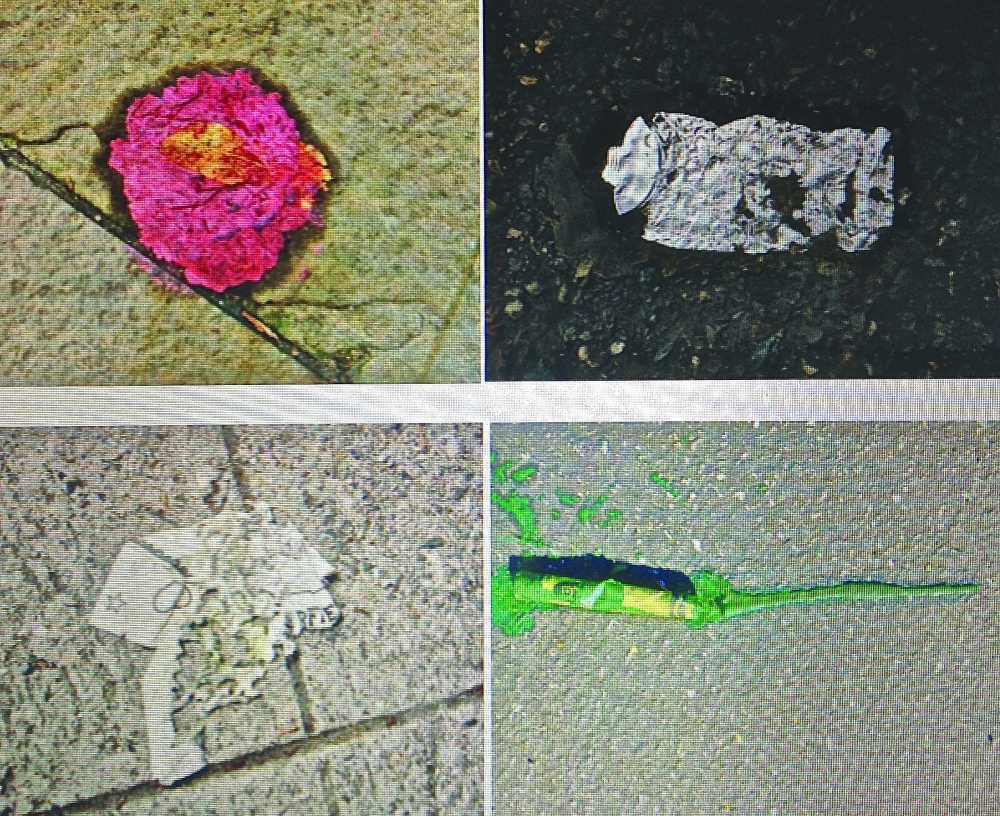
\includegraphics[width=0.8\textwidth]{graphics/FilomenaCruz_RoadKill_ReVista.jpg}
      \caption{Road Kill by Filomena Cruz}
      \label{fig:FilomenaCruz_RoadKill_ReVista}
  \end{figure}

\item Vic Muniz creates monumental trash art in Jardim Gramacho with the help of \textit{catadores} (Waste Land, 2010)

% https://www.youtube.com/watch?v=sJxxdQox7n0
\item Favio Chávez and Nicolás Gómez decide to build musical instruments out of garbage and get 35 children from Cateura, Paraguay’s biggest trash dump, to travel the world with their “Recycled Orchestra,” or “Landfill Harmonic”.

% http://www.eloisacartonera.com.ar/ENGversion.html
\item “Eloísa Cartonera,” a work cooperative in Buenos Aires, proudly produces handmade books with cardboard covers: \quotes{We purchase [\ldots] cardboard from the
urban pickers (\textit{cartoneros}) who pick it from the streets. Our books are on Latin American literature, the most beautiful we had a chance to read in our lives.} \quotes{Some of them are preserved as art books at university libraries, while others circulate as literary pieces expected to disintegrate in time---something anticipated of the material they are made from.} [from PAOLA IBARRA, ReVista]
  \begin{figure}[ht]
      \centering
      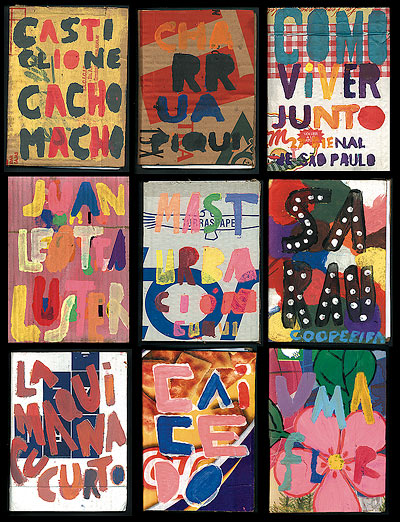
\includegraphics[width=0.8\textwidth]{graphics/EloisaCartonera_Books.jpg}
      \caption{Books covered by Eloisa Cartonera}
      \label{fig:EloisaCartonera_Books}
  \end{figure}

% FROM Paola Ibarra, ReVista
%\item Forever; Blue Yonder by artist Kyle Huffman
%\item Too Too---Much Much by Thomas Hirschhorn
%\item Autoconstrucción by Abraham Cruzvillegas
%\item Pictures of Garbage by Vik Muniz

% FROM Daniel Lind-Ramos BY LOWELL FIET, ReVista
%\item Daniel Lind-Ramos

% FROM A Present from the Sea BY SONIA CABANILLAS, ReVista
% https://www.youtube.com/watch?v=v6IoEF_Tsrw
\item Nick Quijano has some rules to create assemblages. \quotes{There are certain self-imposed rules to this creative process: first, the assemblages or artefactos must all come from material washed ashore on this beach; second, it must be plastic and industrial refuse, result of the processing of fossil fuel; third, it must be polished by a long stay in deep waters, sometimes even encrusted with corals, shells or pebbles, or simply scraped by the ocean floor. As a sign of respect and sacralization, these pieces will be incorporated without any adjustment: no cutting or bending, seen as a mutilation of the object. Its identity cannot be veiled or masked but always must be recognizable amidst the other components; e.g, a comb must remain a comb even as one may see it as a mustache.} The sea returns this refuse; it is not biodegradable.

% FROM Burning Messages BY MICHAEL WELLEN, ReVista
%\item Antonio Berni

% FROM Haiti in the Time of Trash BY LINDA KHACHADURIAN, ReVista
\item Haiti case. When I ask him why he chooses to work in the medium of trash, he replies, \quotes{It gives respect to my city to use the garbage. It shows that everything can be used, and nothing was lost.} (TODO motivation: \quotes{I get more inspiration working with recycled materials because those pieces are unique and can’t be duplicated}) Eugène says that he’s partial to metal, which has become more and more difficult to find because of the clean-up initiative by the city. When I ask him if part of him wishes there were no such effort underway, he answers: \quotes{No. When you have clean streets you have good health, and that is the most important thing.} (This is very strange. It shows that working with trash and being clean healthy is not a contradiction. Both of them exist together.) \quotes{Other people come to Haiti and see junkyards, but we see magical playgrounds,} Jean explains as he watches them.

% FROM Thinking on Film and Trash BY ERNESTO LIVON-GROSMAN, ReVista
% By the 1950s a film like Tire Dié (Fernando Birri, Argentina, 1956) already portrays the collecting, classifying and recycling of trash not only as a source of informal income but as a commercial activity linked to the formal economy. In these films, trash is not the end of a process of consumption but the beginning of a cycle of production. These movies share the idea that trash could be a departure point to think about the modern condition as defined by consumption, class disparities, contamination and urban development. The poet Charles Baudelaire is one of the first to make the connection between the rag picker and the modern city. Walter Benjamin picks it up and from then on the fragmentary condition of trash will remain associated with contemporary art and ultimately with the Modern condition: the industrial refuse could be redeemed by art. It is in this sense that filmmaking becomes allegorical and mimics the process of recycling when it reappropiates archival materials and found footage to create new narratives from scraps, fragments, of films that were not in any way connected to these new narratives.

\end{itemize}

Childs can enjoy with trash. I remember from my childhood, we collect crown cap and play with them. Some caps are found less and they worth more. We are looking everywhere for them. To make them flat we put them on the railways. After train passed we get perfect plat cap. At that time it is not trash for us. It has a value and part of our games and enjoy. To have fun a bunch of trash can be enough for us.

In the case of recycling, a dead objects, or an object that reached end of life will begin a new cycle of life. By the artist or other parts are give them a new life. They can reborn as a different things. Do people collect them aware of it? Discarded items unites together with the hands of a artist. 

Trash is global topic men. When you talk about trash, everyone have ideas about it. 

Think a city that has trash monument in the every corner. created from their trash. merged with the city life and gaining unique cityscapes and aesthetics. or think that a museum a trash museum. Exhibits works of art embracing the trash in all aspects. Maybe done by the artist or the visitors from all around world. A place for garbage other than a landfill. Waiting their creator to meet again. What a great idea isn't it? Meeting their creators again. But this time their creator can recognize their trash. They transformed to totally new thing. Reborn. Transformed (Kafka, Gregor Samsa).

%%
%%
\subsection{Their statements}

%%%
%%%
%%%
\section{My Artwork/Project}

%%
%%
\subsection{Functionality and Art Debate}
From an art historical perspective, you could say that functional art is the inverse of Marcel Duchamp's famous readymades, where he transformed utilitarian objects---a urinal, a bottle rack, etc.---into conceptual artworks by fiat: it became art because he said it was. Duchamp's works kills the functionality. It works beyond the functional perception. Moves the debate to the conceptual frame. However it is not every time case. Today many functional art objects are as avidly acquired by collectors as their fine-art brethren, and are appreciated just as much for their beauty as their use value. Ancient Chinese vases, for example, while still capable of performing their originally intended function (displaying flowers), are prized for their historic and aesthetic value more than anything else. \quotes{In conceptual art,} Sol LeWitt writes, \quotes{the idea or concept is the most important aspect of the work\ldots The idea becomes the machine that makes the art} \cite{lewitt1967paragraphs}. Therefore anything can be turned to art with a good idea. 

%%
%%
\subsection{Paper}
"Paper is an indispensable product throughout the world. Its primary use is as a medium for writing, essential for bureaucracy, education, communications, information storage, and in the spread of information. In addition, it is used for the packaging for transport and convenience of a wide range of items from food to industrial equipment. Paper also has specific technological uses, such as for filters and in art, home furnishings, and architecture, and it has a range of uses for hygiene purposes. Paper in several forms is consumed on a daily basis by each person in the Western world." \cite{trafford2012paper}

%
\subsubsection{Environmental Impact}
Paper is both biodegradable and a renewable resource, which means in consumption and waste terms, its environmental impact is relatively small compared to the many more-toxic and bulky waste products that are found in everyday garbage. However, the chemicals, water, and electricity used in its manufacture are considerable---and these are nonrenewable resources---and certain types of chemicals used in paper production are toxic. In addition, if waste paper is sent to a landfill, it releases carbon dioxide emissions. Further, forest resources are not always as renewable as one may like to think. These environmental impacts can be greatly reduced by recycling (paper being one of the most easily and cheaply recyclable products in everyday use) and by conscientious consumption practices.

Paper made exclusively from wood is called virgin paper, while paper produced out of used paper that is re-pulped is called recycled paper. Recycling paper can greatly diminish demand for virgin fiber from wood. However, there will always be a demand for virgin paper because, although paper is thought of as a renewable resource, it cannot be recycled indefinitely. It can only be recycled four to six times, as the fibers get shorter and weaker each time. In addition, some virgin pulp must be introduced into the process each time to maintain the strength and quality of the fiber, so no matter how much is recycled, paper will always need some virgin fiber.

%
\subsubsection{History}
The word paper comes from papyrus, the plant that was first used for making a medium for writing in ancient Egypt.

%
\subsubsection{Production}
All types and qualities of paper share the same basic method of manufacture, including newspaper paper, print paper, and carton used for boxes.

%
\subsubsection{Uses}
Paper has become the most ubiquitous product in the age of information. Such products often complete their journey from shop floor to garbage in a single day; for example, newspapers, print paper, packaging, lavatory paper, tea bags, transport tickets, price tags, shopping bags, flyers, leaflets, wrapping paper, napkins, and tissues. 

%%
%%
\subsection{Why (package) paper?}
Easy to collect. Easy to find. Thrown out even if it is good quality. Packaging materials are very widespread. Appropriate for painting and writing.

%%
%%
\subsection{Why covering notebooks and books?}

%%
%%
\subsection{Artistic tactics}
Spreading the idea by making something useful and easy to carry while traveling. Small notebooks.  

%%%
%%%
%%%
\section{Literature review, discussions, ideas\ldots}
Trash art is not collage (assemblage or found object) or fragments. it is more than that. The carried messages through the medium have different meaning. It has relationship with activism, craftivism. It refuses consumption based life cycle. It suggests a life practice.

"Every day, we put unwanted material in toilets and garbage bins, regularly flushing it away or taking it out in bags to be transported far away from our homes by others. The names we give this material---waste, garbage, refuse, trash, rubbish--- have pejorative definitions. Worthless. Rejected and useless matter of any kind. Unimportant." "Our trash is a testament; what we throw away says much about our values, our habits, and our lives." "While dictionary definitions of garbage describe it as “filth” and “worthless,” scholars are careful to note that perceptions of waste and the value of material are neither static nor universally shared." "\ldots the question of who owns these discards is not trivial." "The absence of a waste stream aroused suspicion, just as the presence of particular items tell us about the habits of the consumers who generate a waste stream. Our trash is part of us, whether or not we choose to acknowledge it." \cite{zimring2012encyclopedia}

%%
%%
\subsection{Culture, Values, and Garbage}
"The Trash Talk project emphasizes the complex, yet overlooked, relationships that garbage and people share. In terms of their relationship to garbage, all people interact with it on two levels. One is a material connection, indicative of the physical and sensory contacts that people have with garbage. In some households, this connection begins with an individual removing an item from packaging, disposing of that item in the kitchen receptacle, placing that item and others into a larger bin, taking that bin to the curbside, and then the material connection ends. Others, including workers in sanitation plants and recycling centers, then continue a material connection with the garbage, but the material connection of the consumer and the garbage ends with the bin on the curbside. The second connection that people maintain with garbage is an ideational one. Unlike the material one, which is manifested in things that can be touched, moved, and sensed, the ideational connection operates on the level of cognition. The differentiation of an item of value from an item of trash, for example, has nothing to do with the material principles of the object. Instead, humans determine whether the object is of value or whether it is considered trash. The decision of whether an individual decides to dispose of a broken radio or to consider it an heirloom to be kept is highly subjective and rooted in the value systems of a culture." "After the item is eaten, the individual has to decide what to do with the remainder, such as the leftover package. The package might be reused, re-purposed, or recycled but, most likely, will be disposed of in the trash." \cite{lukas2012culture}

%%
%%
\subsection{Garbage Art}
"Garbage art (alternatively known as trash art or recycled art) is art created from materials including post-consumer and other waste, collected debris, or objects previously used for other purposes." "Creating art from garbage involves transforming the meaning of objects by placing them in new, aestheticized contexts. This practice is not new; tribal peoples have adapted bits of trash from industrialized societies into their traditional arts since coming into contact with products of the developed world." "Creating art from trash involves “consuming” garbage in the sense that artists appropriate and rearrange the materials in personal ways, transform their meanings, utilize them to their own ends, and represent them in new ways.It involves taking unwanted materials out of their “waste” context and recontextualizing them as “art.”" \cite{tauxe2012encyclopedia}

%%
%%
\subsection{Garbage in Modern Thought}
"Philosophers and intellectuals have expressed the need to focus on the centrality of garbage, but for everyday individuals, the understanding of garbage is often as something “out of sight, out of mind.”" "Modern humans, as part of their penchant for consumption and unsustainable living, often think very little about the waste that they produce." "Like many aspects of capitalist living, the person throwing away a piece of trash does not connect the various levels of production, consumption, and post-consumption involved in the trash. It becomes a secondary matter---an afterthought." "Martin O’Brien, among many thinkers, argues that the understanding of garbage should be a central concept, especially since garbage typically correlates with social change, social roles, and institutions. Thus, beyond the level of individuals and their relationship to garbage, there is an interest in understanding the central role that garbage plays in all of society’s roles, institutions, and forms of change." "Garbage is excess--- it is a part of society that society no longer desires." \cite{lukas2012garbage}

%
\subsubsection{Categorization and Value}
"Garbage is categorization, according to Susan Strasser." "In recycling programs and in places of refuse disposal, items of trash are categorized depending on their potential value, possible environmental harm, or time of decay. Consumers have become accustomed to the categories that are often applied to garbage. Many cities require people to dispose of their garbage in an orderly fashion---perhaps separating wet household waste from dry---and recycling programs ask individuals to divide their recyclable items into sets (such as plastic, glass, aluminum, and paper) and smaller subsets (such as PET or 01, PE-HD or 02, and PVC or 03). Garbage is an illustration of how humans use mental categories to order the material world." \cite{lukas2012garbage}

"According to John Scanlon, garbage is indicative of a separation of the world---the desirable from the unwanted. Michael Thompson uses the riddle of the rich and poor person’s approach to snot (one keeps his in a handkerchief, the other disposes of it with a tissue) to underscore the curious ways in which garbage is connected to the issue of value. While garbage is universal---all societies, extinct and extant, have produced or produce garbage--- the conditions under which garbage is understood are culturally determined. Many non-Western societies attach a much greater value to items after they are discarded. In the United States and many other nations, garbage often results not because something no longer has utilitarian value but because the item in question is defined as something of no value. Thus, garbage is not only an objective condition of material culture, but also a subjective one of mentalist culture. People define what is trash and what is valuable." \cite{lukas2012garbage}

%
\subsubsection{Semiotic Context}
"In popular writing (such as novels), in television, films, music, and other forms of mass expression, the term trash is used to signify work that is of especially low value." \cite{lukas2012garbage}

%%%
%%%
%%%
\section{Archaeology of Garbage}

%%
%%
\subsection{Garbology}
"Weberman infamously used techniques of what he deemed garbology to uncover what he saw as the essential nature of people. He once said, perhaps indirectly referencing Jean Brillat-Savarin’s quote about food, “You are what you throw away.”" \cite{lukas2012garbage}

"The field of garbology involves the study of refuse and waste. It enables researchers to document information on the nature and changing patterns of modern refuse, hence assisting in the study of contemporary human society or culture. According to the Oxford English Dictionary, the term was first used by waste collectors in the 1960s. A. J. Weberman popularized the term in describing his study of Bob Dylan’s garbage in 1970. It was pioneered as an academic discipline by William Rathje at the University of Arizona in 1973."

In his book “Garbology: Our Dirty Love Affair With Trash”, the Pulitzer prize-winning author Edward Humes notes that other wealthy countries with high living standards have rejected the disposable products that make up much of America's rubbish.

%%
%%
\subsection{Trash as History/Memory}
Walter Benjamin's trash aesthetics and Adornos reflection. \cite{bullock2012trash}

%%
%%
\subsection{Trash Aesthetics}

\bibliographystyle{apacite}
\bibliography{ref}

\end{document}